\documentclass[standalone]{beamer}

\begin{document}
\section{Introduction}

\begin{frame}{{\secname} -- 自我介紹}
\begin{problem}[Roller Coaster Railroad, IOI 2016]
  \small
  現在有 $n$ 段雲霄飛車軌道,你要將這些軌道做排列,並用一些額外的煞車軌道連接他們。
  每段軌道有兩個值 $s_i$, $t_i$ 表示進入這段軌道時車速不能超過 $s_i$,
  且出去這段軌道車速會變為 $t_i$。每一單位長的煞車軌道可以將車子減速一單位,
  請找一個將所有軌道都用到並合乎規定、且用的煞車軌道長度總合最短的方案。($n \leq 2 \cdot 10^5$)
\end{problem}
\pause

\begin{figure}
\includegraphics[width=0.3\textwidth]{figure/bbg.jpg}%
\end{figure}
\end{frame}

\begin{frame}{{\secname} -- 自我介紹}
  \begin{enumerate}
    \item 字串
    \item 圖論、flow
    \item 數學
    \item<2-> 還是數學…
  \end{enumerate}

  \visible<3->{
    \begin{figure}
    \includegraphics[width=0.6\textwidth]{figure/course_match.png}%
    \end{figure}
  }
\end{frame}

\begin{frame}{{\secname} -- 視力檢查}
  \begin{itemize}
    \item<+-> {\fontsize{60pt}{100pt}\selectfont >} \\[20pt]
    \item<+-> {\Huge $\sqcup$} \\[10pt]
    \item<+-> {\Large $\epsilon$} \\[10pt]
    \item<+-> {\Large $\lessgtr$} \\[10pt]
    \item<+-> {\Huge $\ast$}
  \end{itemize}
\end{frame}

\begin{frame}{\secname -- 數學}
  程式競賽中的數學:

  \begin{enumerate}
    \setlength{\itemindent}{2em}
    \item 數學想法
    \item 數學知識
  \end{enumerate}
\end{frame}

\begin{frame}{{\secname} -- 數學想法}
  \begin{problem}[Increasing Numbers, AtCoder Grand Contest 011]
    我們說一個數字是\emph{遞增數},如果他的任意兩個相鄰的位數 $d_i, d_{i+1}$
    都滿足 $d_i \leq d_{i+1}$。給你一個數 $N$,請你把他寫成最少的遞增數的和。
    ($\log_{10} N \leq 5 \cdot 10^5$)
  \end{problem} 
  \pause

  \begin{figure}
    \includegraphics[width=0.5\textwidth]{figure/angry2.png}
  \end{figure}
\end{frame}

\begin{frame}{{\secname} -- 題解}
  \begin{enumerate}
    \item<+-> 關鍵的第一步:
      \visible<+->{ 乘 $9$ 。}
    \item $111\dots111 \times 9 = 999\dots999 = 10^k - 1$
  \end{enumerate}
\end{frame}

\begin{frame}{\secname -- 數學想法}
  \begin{problem}[完全圖的分解]
    給你一個完全圖 $K_{2n}$,請你將所有邊分解成 $n$ 個不相交的 Hamilton Path
    (通過所有點恰一次的鍊)。
  \end{problem}
  \medskip
  \pause

  \begin{columns}
  \column{0.5\textwidth}
    \begin{figure}
    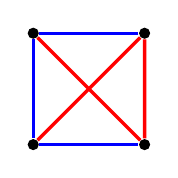
\begin{tikzpicture}[
        nd/.style={fill=black, circle, minimum size=0.1pt, inner sep=0.5mm},
        ed/.style={very thick}
      ]
      \newdimen\R
      \R=1cm
      \foreach \x [count=\i] in {45,135,225,315} { 
        \node[nd] (v\i) at (\x:\R) {}; 
      }
      \draw[ed, blue] (v1) -- (v2) -- (v3) -- (v4);
      \draw[ed, red] (v2) -- (v4) -- (v1) -- (v3);
    \end{tikzpicture}
    \end{figure}
  \column{0.5\textwidth}
    \begin{figure}
    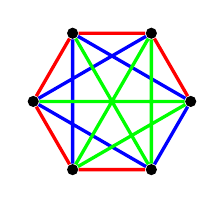
\begin{tikzpicture}[
        nd/.style={fill=black, circle, minimum size=0.1pt, inner sep=0.5mm},
        ed/.style={very thick}
      ]
      \newdimen\R
      \R=1cm
      \foreach \x [count=\i] in {0,60,120,...,300} { 
        \node[nd] (v\i) at (\x:\R) {}; 
      }
      \draw[ed, red] (v1) -- (v2) -- (v3) -- (v4) -- (v5) -- (v6);
      \draw[ed, blue] (v2) -- (v4) -- (v6) -- (v1) -- (v3) -- (v5);
      \draw[ed, green] (v3) -- (v6) -- (v2) -- (v5) -- (v1) -- (v4);
    \end{tikzpicture}
    \end{figure}
  \end{columns}
\end{frame}


\begin{frame}{\secname -- 震驚!}
    \begin{figure}
    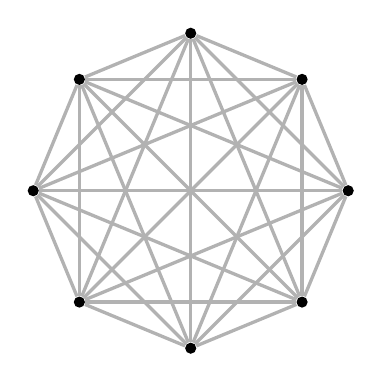
\begin{tikzpicture}[
        nd/.style={fill=black, circle, minimum size=0.1pt, inner sep=0.5mm},
        ed/.style={very thick}
      ]
      \newdimen\R
      \R=2cm
      \foreach \x [count=\i] in {0,45,...,315} { 
        \node[nd] (v\i) at (\x:\R) {}; 
      }
      \foreach \x in {1,...,8} { 
        \foreach \y in {\x,...,8} { 
          \draw[ed, black!30] (v\x) -- (v\y);
        }
      }
    \end{tikzpicture}
    \end{figure}
\end{frame}

\begin{frame}{\secname \ -- 數學知識}
  \begin{problem}[平方國的平方幣, TIOJ 1349]
    給你一個正整數 $n$,請找出最小的 $k$,使得存在 $k$ 個平方數 $a_1^2, a_2^2, \cdots, a_k^2$
    使得 $\sum a_i^2 = n$ 。($n \leq 10^7$)
  \end{problem}

  \begin{itemize}
    \item<2-> 一個很極端的「結論題」。
    \item<3-> 所有正整數都可以寫成 $4$ 個平方數的和。
    \item<4-> 太結論也不是很有趣……
  \end{itemize}
\end{frame}

\begin{frame}{\secname \ -- 數學知識真實案例}
  \begin{problem}[Little Artem and Graph, {\scriptsize VK Cup 2016 Round 2, Div. 1 pF}]
    有一個圖是這樣生成的,從一個 $k$ 個點的完全圖開始,每一次加入一個點,
    連接到 $k$ 個已經在圖上的點。請計算這個圖的生成樹數量。($n \leq 10000$, $k \leq 5$)
  \end{problem}
  \pause

  \begin{itemize}[<+->]
    \item 本來是個 DP 題。
    \item 硬被玩成數學題!
  \end{itemize}
\end{frame}

\begin{frame}{\secname \ -- 怪怪的解法}
  \pause
  \begin{enumerate}[<+->]
    \item 矩陣樹定理。
    \item Cayley–Hamilton theorem,最小多項式求行列式。
    \item Berlekamp-Massey algorithm 求最小多項式。
    \item ???
    \item Profit
  \end{enumerate}
  \pause

  \begin{figure}
    \includegraphics[width=0.9\textwidth]{figure/profit.png}
  \end{figure}
\end{frame}

\begin{frame}{\secname \ -- 數學知識}
  \begin{problem}[經典問題]
    給你 $N$ 個點 $(x_i, y_i)$ ,求一條線 $y = f(x)$ 使得
    \[ \sum_{i = 1}^N (f(x_i) - y_i)^2 \]
    最小。 
  \end{problem}
  \pause

  \begin{figure}
    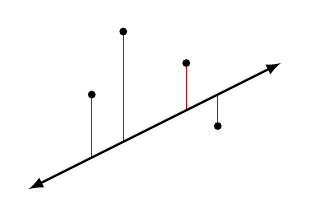
\begin{tikzpicture}[
          nd/.style={fill=black, circle, minimum size=0.1pt, inner sep=0.35mm},
          ed/.style={line width=0.12mm, red!80!black},
          x=4mm,
          y=4mm,
        ]
      \draw[ed] (-1, 1) -- (-1, -1);
      \draw[ed] (0, 3) -- (0, -0.5);
      \draw[ed] (2, 2) -- (2, 0.5);
      \draw[ed] (3, 0) -- (3, 1);
      \draw[latex-latex, thick] (-3, -2) -- (5, 2);
      \node[nd] at (-1, 1) {}; 
      \node[nd] at (0, 3) {}; 
      \node[nd] at (2, 2) {}; 
      \node[nd] at (3, 0) {}; 
    \end{tikzpicture}
  \end{figure}
\end{frame}

\begin{frame}{\secname \ -- 數學知識}
  \begin{problem}[經典問題]
    給你 $N$ 個點 $(x_i, y_i)$ ,求一條線 $y = f(x)$ 使得
    每個點到直線最短矩離的平方和最小。 
  \end{problem}
  \pause

  \begin{figure}
    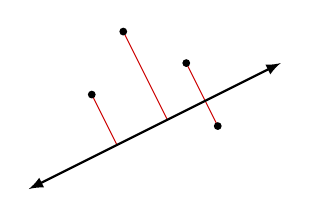
\begin{tikzpicture}[
          nd/.style={fill=black, circle, minimum size=0.1pt, inner sep=0.35mm},
          ed/.style={line width=0.12mm, red!80!black},
          x=4mm,
          y=4mm,
        ]
      \draw[ed] (-1, 1) -- (-0.2, -0.6);
      \draw[ed] (0, 3) -- (1.4, 0.2);
      \draw[ed] (2, 2) -- (3, 0);
      \draw[latex-latex, thick] (-3, -2) -- (5, 2);
      \node[nd] at (-1, 1) {}; 
      \node[nd] at (0, 3) {}; 
      \node[nd] at (2, 2) {}; 
      \node[nd] at (3, 0) {}; 
    \end{tikzpicture}
  \end{figure}
\end{frame}
\end{document}
